\documentclass[openany]{book}
\usepackage{lmodern}
\usepackage{amssymb,amsmath}
\usepackage{ifxetex,ifluatex}
\usepackage{fixltx2e} % provides \textsubscript
\ifnum 0\ifxetex 1\fi\ifluatex 1\fi=0 % if pdftex
  \usepackage[T1]{fontenc}
  \usepackage[utf8]{inputenc}
\else % if luatex or xelatex
  \ifxetex
    \usepackage{mathspec}
  \else
    \usepackage{fontspec}
  \fi
  \defaultfontfeatures{Ligatures=TeX,Scale=MatchLowercase}
\fi
% use upquote if available, for straight quotes in verbatim environments
\IfFileExists{upquote.sty}{\usepackage{upquote}}{}
% use microtype if available
\IfFileExists{microtype.sty}{%
\usepackage{microtype}
\UseMicrotypeSet[protrusion]{basicmath} % disable protrusion for tt fonts
}{}
\usepackage{hyperref}
\hypersetup{unicode=true,
            pdftitle={D3 for R Users},
            pdfauthor={Joyce Robbins},
            pdfborder={0 0 0},
            breaklinks=true}
\urlstyle{same}  % don't use monospace font for urls
\usepackage{natbib}
\bibliographystyle{apalike}
\usepackage{color}
\usepackage{fancyvrb}
\newcommand{\VerbBar}{|}
\newcommand{\VERB}{\Verb[commandchars=\\\{\}]}
\DefineVerbatimEnvironment{Highlighting}{Verbatim}{commandchars=\\\{\}}
% Add ',fontsize=\small' for more characters per line
\usepackage{framed}
\definecolor{shadecolor}{RGB}{248,248,248}
\newenvironment{Shaded}{\begin{snugshade}}{\end{snugshade}}
\newcommand{\AlertTok}[1]{\textcolor[rgb]{0.94,0.16,0.16}{#1}}
\newcommand{\AnnotationTok}[1]{\textcolor[rgb]{0.56,0.35,0.01}{\textbf{\textit{#1}}}}
\newcommand{\AttributeTok}[1]{\textcolor[rgb]{0.77,0.63,0.00}{#1}}
\newcommand{\BaseNTok}[1]{\textcolor[rgb]{0.00,0.00,0.81}{#1}}
\newcommand{\BuiltInTok}[1]{#1}
\newcommand{\CharTok}[1]{\textcolor[rgb]{0.31,0.60,0.02}{#1}}
\newcommand{\CommentTok}[1]{\textcolor[rgb]{0.56,0.35,0.01}{\textit{#1}}}
\newcommand{\CommentVarTok}[1]{\textcolor[rgb]{0.56,0.35,0.01}{\textbf{\textit{#1}}}}
\newcommand{\ConstantTok}[1]{\textcolor[rgb]{0.00,0.00,0.00}{#1}}
\newcommand{\ControlFlowTok}[1]{\textcolor[rgb]{0.13,0.29,0.53}{\textbf{#1}}}
\newcommand{\DataTypeTok}[1]{\textcolor[rgb]{0.13,0.29,0.53}{#1}}
\newcommand{\DecValTok}[1]{\textcolor[rgb]{0.00,0.00,0.81}{#1}}
\newcommand{\DocumentationTok}[1]{\textcolor[rgb]{0.56,0.35,0.01}{\textbf{\textit{#1}}}}
\newcommand{\ErrorTok}[1]{\textcolor[rgb]{0.64,0.00,0.00}{\textbf{#1}}}
\newcommand{\ExtensionTok}[1]{#1}
\newcommand{\FloatTok}[1]{\textcolor[rgb]{0.00,0.00,0.81}{#1}}
\newcommand{\FunctionTok}[1]{\textcolor[rgb]{0.00,0.00,0.00}{#1}}
\newcommand{\ImportTok}[1]{#1}
\newcommand{\InformationTok}[1]{\textcolor[rgb]{0.56,0.35,0.01}{\textbf{\textit{#1}}}}
\newcommand{\KeywordTok}[1]{\textcolor[rgb]{0.13,0.29,0.53}{\textbf{#1}}}
\newcommand{\NormalTok}[1]{#1}
\newcommand{\OperatorTok}[1]{\textcolor[rgb]{0.81,0.36,0.00}{\textbf{#1}}}
\newcommand{\OtherTok}[1]{\textcolor[rgb]{0.56,0.35,0.01}{#1}}
\newcommand{\PreprocessorTok}[1]{\textcolor[rgb]{0.56,0.35,0.01}{\textit{#1}}}
\newcommand{\RegionMarkerTok}[1]{#1}
\newcommand{\SpecialCharTok}[1]{\textcolor[rgb]{0.00,0.00,0.00}{#1}}
\newcommand{\SpecialStringTok}[1]{\textcolor[rgb]{0.31,0.60,0.02}{#1}}
\newcommand{\StringTok}[1]{\textcolor[rgb]{0.31,0.60,0.02}{#1}}
\newcommand{\VariableTok}[1]{\textcolor[rgb]{0.00,0.00,0.00}{#1}}
\newcommand{\VerbatimStringTok}[1]{\textcolor[rgb]{0.31,0.60,0.02}{#1}}
\newcommand{\WarningTok}[1]{\textcolor[rgb]{0.56,0.35,0.01}{\textbf{\textit{#1}}}}
\usepackage{longtable,booktabs}
\usepackage{graphicx,grffile}
\makeatletter
\def\maxwidth{\ifdim\Gin@nat@width>\linewidth\linewidth\else\Gin@nat@width\fi}
\def\maxheight{\ifdim\Gin@nat@height>\textheight\textheight\else\Gin@nat@height\fi}
\makeatother
% Scale images if necessary, so that they will not overflow the page
% margins by default, and it is still possible to overwrite the defaults
% using explicit options in \includegraphics[width, height, ...]{}
\setkeys{Gin}{width=\maxwidth,height=\maxheight,keepaspectratio}
\IfFileExists{parskip.sty}{%
\usepackage{parskip}
}{% else
\setlength{\parindent}{0pt}
\setlength{\parskip}{6pt plus 2pt minus 1pt}
}
\setlength{\emergencystretch}{3em}  % prevent overfull lines
\providecommand{\tightlist}{%
  \setlength{\itemsep}{0pt}\setlength{\parskip}{0pt}}
\setcounter{secnumdepth}{5}
% Redefines (sub)paragraphs to behave more like sections
\ifx\paragraph\undefined\else
\let\oldparagraph\paragraph
\renewcommand{\paragraph}[1]{\oldparagraph{#1}\mbox{}}
\fi
\ifx\subparagraph\undefined\else
\let\oldsubparagraph\subparagraph
\renewcommand{\subparagraph}[1]{\oldsubparagraph{#1}\mbox{}}
\fi

%%% Use protect on footnotes to avoid problems with footnotes in titles
\let\rmarkdownfootnote\footnote%
\def\footnote{\protect\rmarkdownfootnote}

%%% Change title format to be more compact
\usepackage{titling}

% Create subtitle command for use in maketitle
\providecommand{\subtitle}[1]{
  \posttitle{
    \begin{center}\large#1\end{center}
    }
}

\setlength{\droptitle}{-2em}

  \title{D3 for R Users}
    \pretitle{\vspace{\droptitle}\centering\huge}
  \posttitle{\par}
    \author{Joyce Robbins}
    \preauthor{\centering\large\emph}
  \postauthor{\par}
      \predate{\centering\large\emph}
  \postdate{\par}
    \date{2019-11-05}

\usepackage{booktabs}

\begin{document}
\maketitle

{
\setcounter{tocdepth}{1}
\tableofcontents
}
\hypertarget{note-to-readers}{%
\chapter*{Note to readers }\label{note-to-readers}}
\addcontentsline{toc}{chapter}{Note to readers }

This guide adapts Scott Murray's \href{https://www.amazon.com/Interactive-Data-Visualization-Web-Introduction/dp/1491921285/}{\emph{Interactive Data Visualization for the Web, 2nd edition}}--a required text for GR5702--for the needs of this course. Be sure to get the second edition, which is a comprehensive update to D3 version 4. The first edition uses D3 version 3, which is not compatible. (To add to the complication, the current version of D3 is v5. However, since differences between v4 and v5 are minimal, unless otherwise indicated in this guide, the code in \emph{IDVW2} will work with either.)

We rely on the text heavily but also deviate from it in several ways. \emph{IDVW2} is written for graphics designers not data science students so the pain points are somewhat different.

In terms of content, we will use certain ES6 conventions not covered in \emph{IDVW2} that make coding easier (and more like R!). We use different examples, though you are strongly encouraged to study \href{https://github.com/alignedleft/d3-book/releases}{Murray's code examples} in addition to reading the text. Particularly through the first half, we don't follow the text in order, so always refer to this guide first which will direct you to the pages of the text that you should read.

This is very much a work-in-progress so please \href{https://github.com/jtr13/d3book/issues}{submit issues} on GitHub to provide feedback and edit or add text by submitting pull requests. (Click the icon at the top of each page to get started. More \href{https://edav.info/contribute.html\#step-2-click-the-edit-button}{detailed instructions} are available on edav.info.)

\hypertarget{jump}{%
\chapter{Jump in the deep end }\label{jump}}

Let's skip the explanations and start coding in D3 right now. Why? So you can see the benefits and know what you're working toward when you get stuck in the weeds. Then we'll go back and start learning step by step.

\hypertarget{get-ready}{%
\section{Get ready }\label{get-ready}}

\begin{enumerate}
\def\labelenumi{\arabic{enumi}.}
\item
  If you don't have it already, download the \href{https://www.google.com/chrome/}{Chrome browser}.
\item
  Download a copy of \texttt{shapes.html}: open the following page and then click \emph{File, Save Page As\ldots{}}: \href{https://raw.githubusercontent.com/jtr13/d3book/master/code/shapes.html}{\texttt{shapes.html}}. (Or download a zip of the whole repo. Clicking \href{https://github.com/jtr13/d3book/archive/master.zip}{here} will start the download. Or fork and clone the \href{https://github.com/jtr13/d3book}{repo}).
\item
  If Chrome is your default browser, open \texttt{shapes.html} by double clicking it. Otherwise, open it with \emph{File, Open File\ldots{}} in Chrome.
\end{enumerate}

\hypertarget{elements-tab}{%
\section{Elements tab }\label{elements-tab}}

\begin{enumerate}
\def\labelenumi{\arabic{enumi}.}
\item
  In Chrome, click \emph{View, Developer, Developer Tools,} then the Elements tab.
\item
  Hover the mouse over various elements in the \texttt{\textless{}body\textgreater{}\ ...\ \textless{}/body\textgreater{}} section. Observe the highlighted sections in the rendered web page on the left of the screen. Click on the mini black triangles to the left of the \texttt{\textless{}body\textgreater{}} and \texttt{\textless{}svg\textgreater{}} tags if needed to open these sections of the DOM tree. Your screen should look like this:
\end{enumerate}

\begin{center}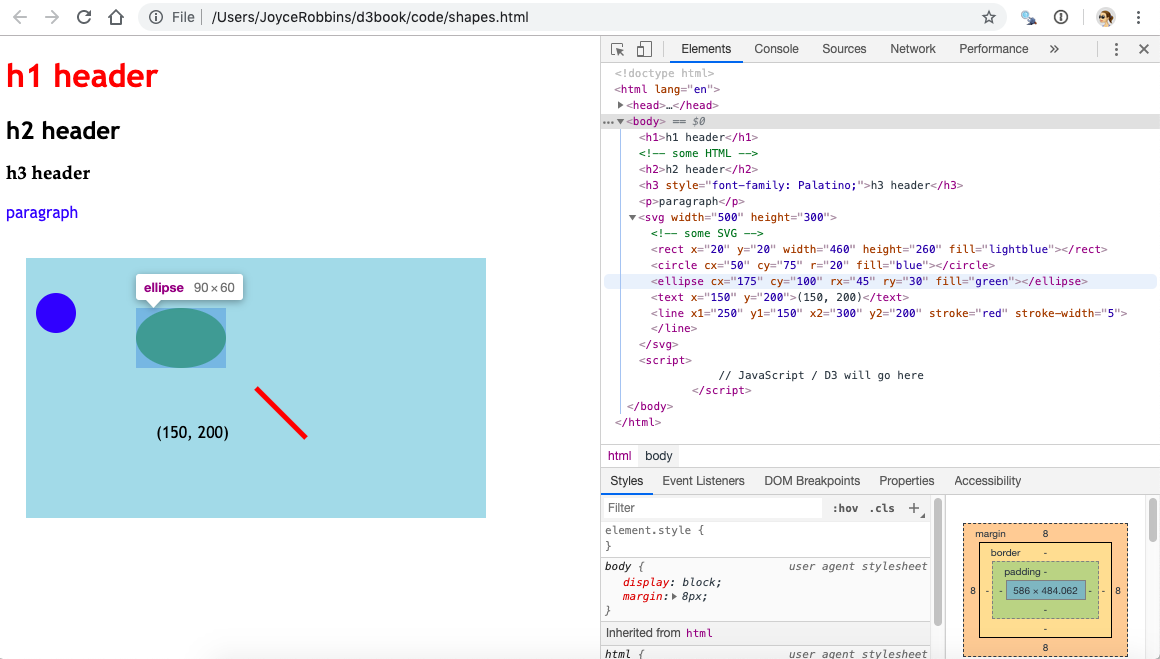
\includegraphics[width=0.8\linewidth]{images/elements} \end{center}

\begin{enumerate}
\def\labelenumi{\arabic{enumi}.}
\setcounter{enumi}{2}
\tightlist
\item
  Now try the reverse: right click on elements on the web page, choose ``Inspect'' and see what is highlighted in the Elements pane. Get comfortable with the connection between the code on the right and the rendered elements on the left.
\end{enumerate}

\hypertarget{console-tab}{%
\section{Console tab }\label{console-tab}}

\begin{enumerate}
\def\labelenumi{\arabic{enumi}.}
\tightlist
\item
  Switch to the Console tab, next to the Elements tab. Let's practice running some code. Note that the code is unrelated to the \texttt{shapes.html} web page that we have open.
\end{enumerate}

\begin{quote}
 \emph{We will spend a lot of time in the Console since it's interactive -- think R console. Eventually we will switch to including JavaScript/D3 in \texttt{.html} or \texttt{.js} files and use the Console only for testing things out or debugging.}
\end{quote}

\begin{enumerate}
\def\labelenumi{\arabic{enumi}.}
\setcounter{enumi}{1}
\tightlist
\item
  Type the following lines of code at the prompt (\texttt{\textgreater{}}), press enter after each line--that is, after the semicolon (\texttt{;})--and see what happens:
\end{enumerate}

\begin{Shaded}
\begin{Highlighting}[]
\DecValTok{3} \OperatorTok{+} \DecValTok{4}\OperatorTok{;}
    
\StringTok{"3"} \OperatorTok{+} \StringTok{"4"}\OperatorTok{;}

\NormalTok{ x }\OperatorTok{=}\NormalTok{ [}\DecValTok{1}\OperatorTok{,} \DecValTok{2}\OperatorTok{,} \DecValTok{3}\NormalTok{]}\OperatorTok{;}
    
\NormalTok{x[}\DecValTok{1}\NormalTok{]}\OperatorTok{;}
    
\NormalTok{x }\OperatorTok{+} \DecValTok{1}\OperatorTok{;}
    
\NormalTok{y }\OperatorTok{=} \OperatorTok{\{}\DataTypeTok{a}\OperatorTok{:} \DecValTok{3}\OperatorTok{,} \DataTypeTok{b}\OperatorTok{:} \DecValTok{4}\OperatorTok{\};}
    
\NormalTok{y[}\StringTok{"b"}\NormalTok{]}\OperatorTok{;}
\end{Highlighting}
\end{Shaded}

\hypertarget{modify-elements}{%
\section{Modify elements }\label{modify-elements}}

\begin{enumerate}
\def\labelenumi{\arabic{enumi}.}
\item
  Now we'll start using D3 to manipulate elements on the page. Try the following, by entering one line at a time in the Console as before:

\begin{Shaded}
\begin{Highlighting}[]
\VariableTok{d3}\NormalTok{.}\AttributeTok{select}\NormalTok{(}\StringTok{"circle"}\NormalTok{).}\AttributeTok{attr}\NormalTok{(}\StringTok{"cx"}\OperatorTok{,} \StringTok{"200"}\NormalTok{)}\OperatorTok{;}

\VariableTok{d3}\NormalTok{.}\AttributeTok{select}\NormalTok{(}\StringTok{"circle"}\NormalTok{).}\AttributeTok{attr}\NormalTok{(}\StringTok{"cx"}\OperatorTok{,} \StringTok{"500"}\NormalTok{)}\OperatorTok{;}

\VariableTok{d3}\NormalTok{.}\AttributeTok{select}\NormalTok{(}\StringTok{"circle"}\NormalTok{).}\AttributeTok{attr}\NormalTok{(}\StringTok{"cx"}\OperatorTok{,} \StringTok{"100"}\NormalTok{)}\OperatorTok{;}

\VariableTok{d3}\NormalTok{.}\AttributeTok{select}\NormalTok{(}\StringTok{"circle"}\NormalTok{).}\AttributeTok{attr}\NormalTok{(}\StringTok{"r"}\OperatorTok{,} \StringTok{"30"}\NormalTok{)}\OperatorTok{;}

\VariableTok{d3}\NormalTok{.}\AttributeTok{select}\NormalTok{(}\StringTok{"circle"}\NormalTok{).}\AttributeTok{attr}\NormalTok{(}\StringTok{"r"}\OperatorTok{,} \StringTok{"130"}\NormalTok{)}\OperatorTok{;}

\VariableTok{d3}\NormalTok{.}\AttributeTok{select}\NormalTok{(}\StringTok{"circle"}\NormalTok{).}\AttributeTok{attr}\NormalTok{(}\StringTok{"r"}\OperatorTok{,} \StringTok{"3"}\NormalTok{)}\OperatorTok{;}

\VariableTok{d3}\NormalTok{.}\AttributeTok{select}\NormalTok{(}\StringTok{"circle"}\NormalTok{).}\AttributeTok{attr}\NormalTok{(}\StringTok{"fill"}\OperatorTok{,} \StringTok{"red"}\NormalTok{)}\OperatorTok{;}

\VariableTok{d3}\NormalTok{.}\AttributeTok{select}\NormalTok{(}\StringTok{"circle"}\NormalTok{).}\AttributeTok{attr}\NormalTok{(}\StringTok{"fill"}\OperatorTok{,} \StringTok{"aliceblue"}\NormalTok{)}\OperatorTok{;}

\VariableTok{d3}\NormalTok{.}\AttributeTok{select}\NormalTok{(}\StringTok{"circle"}\NormalTok{).}\AttributeTok{attr}\NormalTok{(}\StringTok{"fill"}\OperatorTok{,} \StringTok{"lightseagreen"}\NormalTok{)}\OperatorTok{;}
\end{Highlighting}
\end{Shaded}
\end{enumerate}

\begin{quote}
 \emph{Note that ``select'' and ``attr'' are separate operations chained together with ``.'' -- think pipe (\%\textgreater{}\%) operator.}
\end{quote}

\begin{enumerate}
\def\labelenumi{\arabic{enumi}.}
\setcounter{enumi}{1}
\item
  Refresh the page. What happened?
\item
  Go to Elements. Look at the value of the \texttt{y1} attribute of the SVG \texttt{\textless{}line\textgreater{}} element. Go back to the Console and enter the following:

\begin{Shaded}
\begin{Highlighting}[]
\VariableTok{d3}\NormalTok{.}\AttributeTok{select}\NormalTok{(}\StringTok{"line"}\NormalTok{).}\AttributeTok{attr}\NormalTok{(}\StringTok{"y1"}\OperatorTok{,} \StringTok{"10"}\NormalTok{)}\OperatorTok{;}
\end{Highlighting}
\end{Shaded}
\item
  Switch back to Elements and observe. What happened?
\item
  Stay in Elements and refresh the page. What happened to \texttt{y1}?
\item
  Return to the Console to make style changes to the HTML elements:

\begin{Shaded}
\begin{Highlighting}[]
\VariableTok{d3}\NormalTok{.}\AttributeTok{select}\NormalTok{(}\StringTok{"h1"}\NormalTok{).}\AttributeTok{style}\NormalTok{(}\StringTok{"color"}\OperatorTok{,} \StringTok{"purple"}\NormalTok{)}\OperatorTok{;}

\VariableTok{d3}\NormalTok{.}\AttributeTok{select}\NormalTok{(}\StringTok{"h2"}\NormalTok{).}\AttributeTok{style}\NormalTok{(}\StringTok{"font-size"}\OperatorTok{,} \StringTok{"50px"}\NormalTok{)}\OperatorTok{;}

\VariableTok{d3}\NormalTok{.}\AttributeTok{select}\NormalTok{(}\StringTok{"h2"}\NormalTok{).}\AttributeTok{style}\NormalTok{(}\StringTok{"font-family"}\OperatorTok{,} \StringTok{"Impact"}\NormalTok{)}\OperatorTok{;}
\end{Highlighting}
\end{Shaded}
\end{enumerate}

\hypertarget{transitions}{%
\section{Transitions }\label{transitions}}

\begin{enumerate}
\def\labelenumi{\arabic{enumi}.}
\item
  Try these:

\begin{Shaded}
\begin{Highlighting}[]
\VariableTok{d3}\NormalTok{.}\AttributeTok{select}\NormalTok{(}\StringTok{"circle"}\NormalTok{).}\AttributeTok{transition}\NormalTok{().}\AttributeTok{duration}\NormalTok{(}\DecValTok{2000}\NormalTok{).}\AttributeTok{attr}\NormalTok{(}\StringTok{"cx"}\OperatorTok{,} \StringTok{"400"}\NormalTok{)}\OperatorTok{;}

\VariableTok{d3}\NormalTok{.}\AttributeTok{select}\NormalTok{(}\StringTok{"ellipse"}\NormalTok{).}\AttributeTok{transition}\NormalTok{().}\AttributeTok{duration}\NormalTok{(}\DecValTok{2000}\NormalTok{).}\AttributeTok{attr}\NormalTok{(}\StringTok{"transform"}\OperatorTok{,} \StringTok{"translate (400, 400)"}\NormalTok{)}\OperatorTok{;}

\VariableTok{d3}\NormalTok{.}\AttributeTok{select}\NormalTok{(}\StringTok{"line"}\NormalTok{).}\AttributeTok{transition}\NormalTok{().}\AttributeTok{duration}\NormalTok{(}\DecValTok{2000}\NormalTok{).}\AttributeTok{attr}\NormalTok{(}\StringTok{"x1"}\OperatorTok{,} \StringTok{"400"}\NormalTok{)}\OperatorTok{;}

\VariableTok{d3}\NormalTok{.}\AttributeTok{select}\NormalTok{(}\StringTok{"line"}\NormalTok{).}\AttributeTok{transition}\NormalTok{().}\AttributeTok{duration}\NormalTok{(}\DecValTok{2000}\NormalTok{).}\AttributeTok{attr}\NormalTok{(}\StringTok{"y1"}\OperatorTok{,} \StringTok{"250"}\NormalTok{)}\OperatorTok{;}

\VariableTok{d3}\NormalTok{.}\AttributeTok{select}\NormalTok{(}\StringTok{"p"}\NormalTok{).}\AttributeTok{transition}\NormalTok{().}\AttributeTok{duration}\NormalTok{(}\DecValTok{2000}\NormalTok{).}\AttributeTok{style}\NormalTok{(}\StringTok{"font-size"}\OperatorTok{,} \StringTok{"72px"}\NormalTok{)}\OperatorTok{;}
\end{Highlighting}
\end{Shaded}
\item
  Experiment with more transitions.
\end{enumerate}

\hypertarget{interactivity}{%
\section{Interactivity }\label{interactivity}}

\begin{enumerate}
\def\labelenumi{\arabic{enumi}.}
\item
  Set up a function to turn the fill color to yellow:

\begin{Shaded}
\begin{Highlighting}[]
\KeywordTok{function} \AttributeTok{goyellow}\NormalTok{() }\OperatorTok{\{}\VariableTok{d3}\NormalTok{.}\AttributeTok{select}\NormalTok{(}\KeywordTok{this}\NormalTok{).}\AttributeTok{attr}\NormalTok{(}\StringTok{"fill"}\OperatorTok{,} \StringTok{"yellow"}\NormalTok{)}\OperatorTok{\};}
\end{Highlighting}
\end{Shaded}
\item
  Add an event listener to the circle that will be trigger a call to \texttt{goyellow()} on a mouseover:

\begin{Shaded}
\begin{Highlighting}[]
\VariableTok{d3}\NormalTok{.}\AttributeTok{select}\NormalTok{(}\StringTok{"circle"}\NormalTok{).}\AttributeTok{on}\NormalTok{(}\StringTok{"mouseover"}\OperatorTok{,}\NormalTok{ goyellow)}\OperatorTok{;}
\end{Highlighting}
\end{Shaded}
\item
  Test it out.
\item
  Add the same event listener to the ellipse. Test it out.
\item
  Create a function \texttt{goblue()} that changes the fill color to blue.
\item
  Add event listeners to the circle and ellipse that will trigger a call to \texttt{goblue()} on a \emph{mouseout}. Test out your code.
\item
  Try out a click event. (Note the use of an anonymous function.)

\begin{Shaded}
\begin{Highlighting}[]
\VariableTok{d3}\NormalTok{.}\AttributeTok{select}\NormalTok{(}\StringTok{"line"}\NormalTok{).}\AttributeTok{on}\NormalTok{(}\StringTok{"click"}\OperatorTok{,} \KeywordTok{function}\NormalTok{()}
  \OperatorTok{\{}\VariableTok{d3}\NormalTok{.}\AttributeTok{select}\NormalTok{(}\KeywordTok{this}\NormalTok{).}\AttributeTok{attr}\NormalTok{(}\StringTok{"stroke-width"}\OperatorTok{,} \StringTok{"10"}\NormalTok{)}\OperatorTok{;\}}\NormalTok{)}\OperatorTok{;}
\end{Highlighting}
\end{Shaded}
\item
  Try another click event. What's happening?

\begin{Shaded}
\begin{Highlighting}[]
\VariableTok{d3}\NormalTok{.}\AttributeTok{select}\NormalTok{(}\StringTok{"svg"}\NormalTok{).}\AttributeTok{on}\NormalTok{(}\StringTok{"click"}\OperatorTok{,} \KeywordTok{function}\NormalTok{()}
  \OperatorTok{\{}\VariableTok{d3}\NormalTok{.}\AttributeTok{select}\NormalTok{(}\StringTok{"text"}\NormalTok{).}\AttributeTok{text}\NormalTok{(}\VerbatimStringTok{`(}\SpecialCharTok{$\{}\VariableTok{d3}\NormalTok{.}\AttributeTok{mouse}\NormalTok{(}\KeywordTok{this}\NormalTok{)}\SpecialCharTok{\}}\VerbatimStringTok{)`}\NormalTok{)}\OperatorTok{\}}\NormalTok{)}\OperatorTok{;}
\end{Highlighting}
\end{Shaded}
\end{enumerate}

Ok, now that we have a taste for what D3 can do, let's break it down, which we'll do in the next chapter.

\hypertarget{web}{%
\chapter{Web tech }\label{web}}

Read: Chapter 3 ``Technology Fundamentals'' (pp.~17-62)

\emph{There is a lot of material in this chapter. It is worth making the effort to learn it now and start D3 with a solid foundation of elementary HTML/CSS/SVG/JavaScript.}

Here we examine \texttt{shapes.html} from Chapter 1 to see how the various technologies are combined into a single document.

\hypertarget{html}{%
\section{HTML }\label{html}}

Note that \texttt{shapes.html} has an HyperText Markup Language or \texttt{.html} extension; HTML in fact provides the structure for the document. It has a \texttt{\textless{}head\textgreater{}} and \texttt{\textless{}body\textgreater{}} section.

In the \texttt{\textless{}head\textgreater{}} section we use \texttt{\textless{}script\textgreater{}} tags to link to the D3 library:

\begin{Shaded}
\begin{Highlighting}[]
\OperatorTok{<}\NormalTok{script src}\OperatorTok{=}\StringTok{"https://d3js.org/d3.v5.min.js"}\OperatorTok{>}\NormalTok{</script}\OperatorTok{>}\VerbatimStringTok{`}
\end{Highlighting}
\end{Shaded}

\hypertarget{css}{%
\section{CSS }\label{css}}

CSS (Cascading Style Sheets) is used for styling web pages, and more importantly for our purposes, selecting elements on a page or in a graphic. We will generally work with internal style sheets since it's simpler when starting out to have everything in one document. External style sheets, however, are generally the preferred method for web design.

\hypertarget{internal-style-sheet}{%
\subsection{Internal style sheet}\label{internal-style-sheet}}

\texttt{shapes.html} has an \emph{internal style sheet}: CSS style information appears in the \texttt{\textless{}head\textgreater{}} section marked off with \texttt{\textless{}style\textgreater{}} tags:

\begin{Shaded}
\begin{Highlighting}[]
\OperatorTok{<}\NormalTok{style type}\OperatorTok{=}\StringTok{"text/css"}\OperatorTok{>}
\NormalTok{    h1 }\OperatorTok{\{}\DataTypeTok{color}\OperatorTok{:}\NormalTok{red}\OperatorTok{;\}}     \CommentTok{/* CSS styling */}
\NormalTok{    p }\OperatorTok{\{}\DataTypeTok{color}\OperatorTok{:}\NormalTok{blue}\OperatorTok{;\}}
\NormalTok{</style}\OperatorTok{>}
\end{Highlighting}
\end{Shaded}

Here we specify that all HTML \texttt{\textless{}h1\textgreater{}} headers should be red and all HTML paragraphs \texttt{\textless{}p\textgreater{}} should be blue. This is an example of an \emph{internal style sheet}. Later we will consider alternatives: \emph{external style sheets} and \emph{inline styling}.

Styling for coder designed classes is also specified in this section. For example, we could style a ``formal'' class as such:

\begin{Shaded}
\begin{Highlighting}[]
\OperatorTok{<}\NormalTok{style type}\OperatorTok{=}\StringTok{"text/css"}\OperatorTok{>}
\NormalTok{    .}\AttributeTok{formal} \OperatorTok{\{}\DataTypeTok{color}\OperatorTok{:}\NormalTok{ red}\OperatorTok{;}        
\NormalTok{        font}\OperatorTok{-}\DataTypeTok{size}\OperatorTok{:}\NormalTok{ 30px}\OperatorTok{;}
\NormalTok{        font}\OperatorTok{-}\DataTypeTok{family}\OperatorTok{:}\NormalTok{ Lucida Calligraphy}\OperatorTok{;}
        \OperatorTok{\}}   
\NormalTok{</style}\OperatorTok{>}
\end{Highlighting}
\end{Shaded}

Note that classes are defined by the ``.'' before the name.

\hypertarget{external-style-sheets}{%
\subsection{External style sheets}\label{external-style-sheets}}

External style sheets are \texttt{.css} files that contain styling information and are linked to with a \texttt{\textless{}link\textgreater{}} tag in the \texttt{\textless{}head\textgreater{}} section of an HTML document:

\begin{Shaded}
\begin{Highlighting}[]
\OperatorTok{<}\NormalTok{head}\OperatorTok{>}
    \OperatorTok{<}\NormalTok{link rel}\OperatorTok{=}\StringTok{"stylesheet"}\NormalTok{ href}\OperatorTok{=}\StringTok{"style.css"}\OperatorTok{>}
\NormalTok{</head}\OperatorTok{>}
\end{Highlighting}
\end{Shaded}

External style sheets are the preferred way of styling as they can easily be modified without changing the web page; in fact, the motivation for CSS came from a desire in the early days of the internet to separate styling from content.

Developers have the option now of choosing premade themes, which are shared through external style sheets. They can be quite complex. The \href{https://github.com/thomaspark/bootswatch/blob/master/docs/4/minty/bootstrap.css}{\texttt{.css} file} for the ~Minty~ theme from Bootswatch, for example, contains over 10,000 lines.

\href{http://www.csszengarden.com/}{CSS Zen Garden} demonstrates the power of external style sheets: the same HTML document takes on very different looks depending on the stylesheet to which it is linked.

\hypertarget{inline-styling}{%
\subsection{Inline styling}\label{inline-styling}}

With inline styling, styling is added to each tag individually:

\begin{verbatim}
<span style="color: white; background-color: fuchsia; font-family: impact; 
      font-size: 24px; border-style: solid; border-color: limegreen; 
      border-width: 3px">
      Styled inline
</span>
\end{verbatim}

This is how early web pages were styled. To take a step back in time, use developer tools to view the source code for the main page of \href{http://www.dolekemp96.org/main.htm}{www.dolekemp96.org}, an old web site that has been maintained for historical purposes. As you can see, it's a tedious way of writing content, which internal and external style sheets eliminate.

Although you will not be adding inline styling manually, you will notice that when we select elements and change the styling with D3, the modifications are made inline. In other words, we do not make changes to the elements directly, not via a style sheet.

\hypertarget{svg}{%
\section{SVG }\label{svg}}

SVG (Scalable Vector Graphics) is a human readable graphics format that facilitates manipulation of individual elements. You may be familiar with \texttt{.svg} files. Here we have SVG graphics within \texttt{\textless{}svg\textgreater{}} tags in the \texttt{\textless{}body\textgreater{}} section of the HTML document:

\begin{Shaded}
\begin{Highlighting}[]
\OperatorTok{<}\NormalTok{svg width}\OperatorTok{=}\StringTok{"500"}\NormalTok{ height}\OperatorTok{=}\StringTok{"300"}\OperatorTok{>}  \OperatorTok{<!--}\NormalTok{ some SVG }\OperatorTok{-->}
    \OperatorTok{<}\NormalTok{rect x}\OperatorTok{=}\StringTok{"20"}\NormalTok{ y}\OperatorTok{=}\StringTok{"20"}\NormalTok{ width}\OperatorTok{=}\StringTok{"460"}\NormalTok{ height}\OperatorTok{=}\StringTok{"260"}\NormalTok{ fill}\OperatorTok{=}\StringTok{"lightblue"}\OperatorTok{>}\NormalTok{</rect}\OperatorTok{>}
    \OperatorTok{<}\NormalTok{circle cx}\OperatorTok{=}\StringTok{"50"}\NormalTok{ cy}\OperatorTok{=}\StringTok{"75"}\NormalTok{ r}\OperatorTok{=}\StringTok{"20"}\NormalTok{ fill}\OperatorTok{=}\StringTok{"blue"}\OperatorTok{>}\NormalTok{</circle}\OperatorTok{>}
    \OperatorTok{<}\NormalTok{ellipse cx}\OperatorTok{=}\StringTok{"175"}\NormalTok{ cy}\OperatorTok{=}\StringTok{"100"}\NormalTok{ rx}\OperatorTok{=}\StringTok{"45"}\NormalTok{ ry}\OperatorTok{=}\StringTok{"30"}\NormalTok{ fill}\OperatorTok{=}\StringTok{"green"}\OperatorTok{>}\NormalTok{</ellipse}\OperatorTok{>}
    \OperatorTok{<}\NormalTok{text x}\OperatorTok{=}\StringTok{"150"}\NormalTok{ y}\OperatorTok{=}\StringTok{"200"}\OperatorTok{>}\NormalTok{(}\DecValTok{150}\OperatorTok{,} \DecValTok{200}\NormalTok{)</text}\OperatorTok{>}
    \OperatorTok{<}\NormalTok{line x1}\OperatorTok{=}\StringTok{"250"}\NormalTok{ y1}\OperatorTok{=}\StringTok{"150"}\NormalTok{ x2}\OperatorTok{=}\StringTok{"300"}\NormalTok{ y2}\OperatorTok{=}\StringTok{"200"}\NormalTok{ stroke}\OperatorTok{=}\StringTok{"red"}\NormalTok{ stroke}\OperatorTok{-}\NormalTok{width}\OperatorTok{=}\StringTok{"5"}\OperatorTok{>}\NormalTok{</line}\OperatorTok{>}
\NormalTok{</svg}\OperatorTok{>}
\end{Highlighting}
\end{Shaded}

Rendered:

`

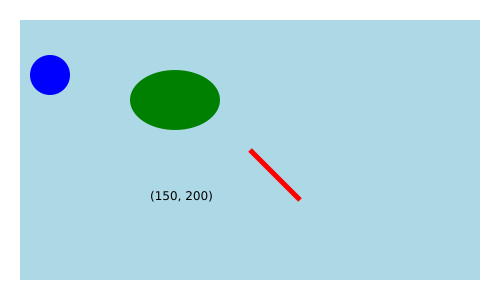
\includegraphics[width=0.5\linewidth]{images/shapessvg}

There are very few SVG tags that you'll need to know, and once we get going with D3, you will not have to code any SVG manually. It is worth doing a little to become familiar with the format and in particular to get used to the new location of the origin.

\hypertarget{javascript}{%
\section{JavaScript }\label{javascript}}

JavaScript is the most common language for making web pages interactive. Code is executed when pages are opened or refreshed. So far we have run JavaScript in the Console, but have not included it in the web page itself. When we do so, it will be between \texttt{\textless{}script\textgreater{}} tags in the \texttt{\textless{}body\textgreater{}} section of the HTML document, or in a separate \texttt{.js} file.

\hypertarget{d3}{%
\section{D3 }\label{d3}}

D3 (Data Driven Documents) is a JavaScript library well suited to interactive graphics. As such, it is also included between \texttt{\textless{}script\textgreater{}} tags in the \texttt{\textless{}body\textgreater{}} section. For D3 to work, you must link to the D3 library in the \texttt{\textless{}head\textgreater{}} section of the document.

There seems to be a misconception that D3 is a high level language. It is not. You will be working on the pixel level to create graphics, including drawing your own axes and doing other things that you're not used to doing if you've been working in R or Python.

\begin{quote}
 \emph{On the bright side, after D3, you will gain a new appreciation for base R graphics. You will write code such as \texttt{plot(iris\$Sepal.Length,\ iris\$Sepal.Width,\ pch\ =\ 16,\ col\ =\ iris\$Species,\ las\ =\ 1,\ xlab\ =\ "Sepal.Length",\ ylab\ =\ "Sepal.Width")} and think: wow, there are axes! Amazing!}
\end{quote}

It is legitimate to ask why you need to know D3 as a data scientist. Many if not most of you will not be coding in JavaScript from the ground up in your future careers. However, it's a great way to learn how interactive graphics work under the hood, and will give you a solid foundation which you can draw on to tweak visualizations that you build with high level tools such as \href{https://plot.ly/}{Plotly}.

\hypertarget{html-tree}{%
\section{HTML tree }\label{html-tree}}

While \texttt{shapes.html} appears as a single consistent document, it is actually comprised of multiple languages. HTML, CSS, and SVG are already there, and we will be adding JavaScript / D3 soon.

\begin{center}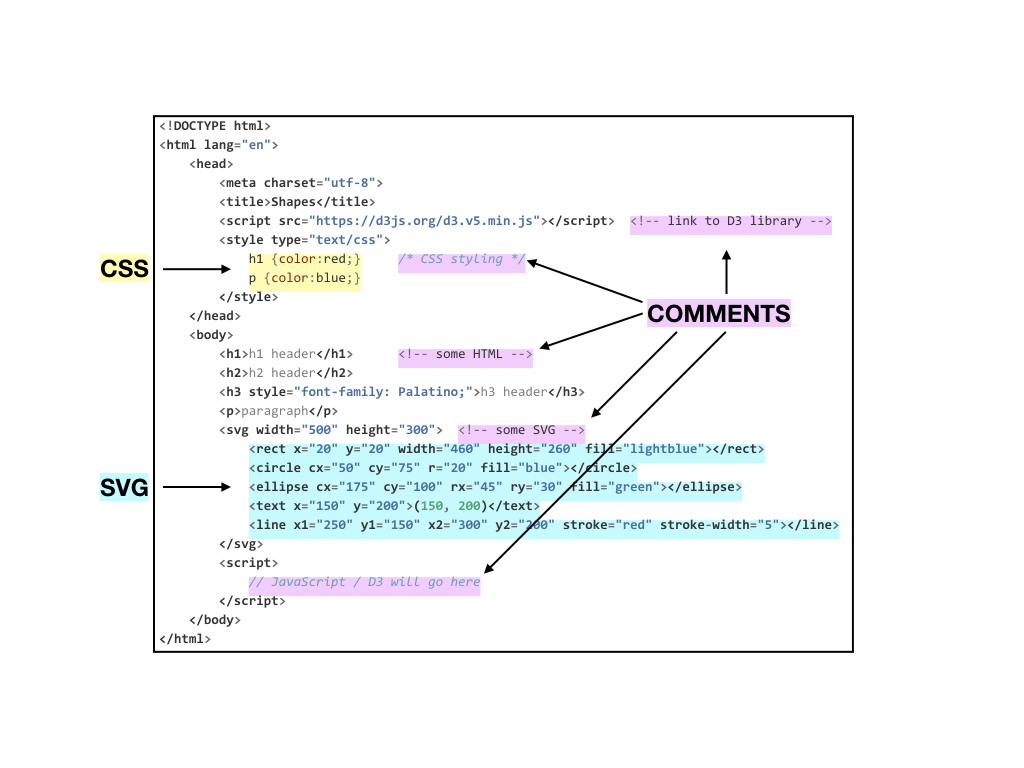
\includegraphics[width=1\linewidth]{images/shapes} \end{center}

Of note:

\begin{itemize}
\item
  An HTML document is composed of lines or sections set off with tags. In particular \texttt{\textless{}style\textgreater{}\ ...\ \textless{}/style\textgreater{}}, \texttt{\textless{}svg\textgreater{}\ ...\ \textless{}/svg\textgreater{}}, and \texttt{\textless{}script\textgreater{}\ ...\ \textless{}/script\textgreater{}} indicate the inclusion of CSS, SVG, and JavaScript/D3 respectively.
\item
  For D3 to work, you must link to a D3 library. Here we link to an online version, but you can also download a copy from \url{https://d3js.org} and reference the local copy with:

\begin{Shaded}
\begin{Highlighting}[]
\OperatorTok{<}\NormalTok{script src}\OperatorTok{=}\StringTok{"d3.js"}\OperatorTok{>}\NormalTok{</script}\OperatorTok{>}
\end{Highlighting}
\end{Shaded}
\item
  Comment syntax varies with language:

  \begin{itemize}
  \item
    \texttt{\textless{}!-\/-\ single\ or\ multiline\ HTML\ or\ SVG\ comment\ -\/-\textgreater{}}
  \item
    \texttt{/*\ single\ or\ multiline\ CSS\ comment\ */}
  \item
    \texttt{//\ single\ line\ JavaScript\ comment}
  \item
    \texttt{/*\ JavaScript} \texttt{multiline\ comment\ */}
  \end{itemize}
\end{itemize}

\hypertarget{exercise}{%
\section{Exercise }\label{exercise}}

Download a fresh copy of \texttt{shapes.html}. (Reminder: open the following page and then click \emph{File, Save Page As\ldots{}}: \href{https://raw.githubusercontent.com/jtr13/d3book/master/code/shapes.html}{\texttt{shapes.html}}). Open the file in a text editor of your choice on one half of your screen. If you don't want to think about it, just use RStudio since it's already installed and provides syntax highlighting for \texttt{.html}. On the other half of your screen open the same file in Chrome. Developer Tools should not be open; we will not be using the Console. As you make changes to the \texttt{.html} file, save the file and then refresh the browser to see the effects. Keyboard shortcuts to save and refresh are helpful here.

Your screen should look like this:

\begin{center}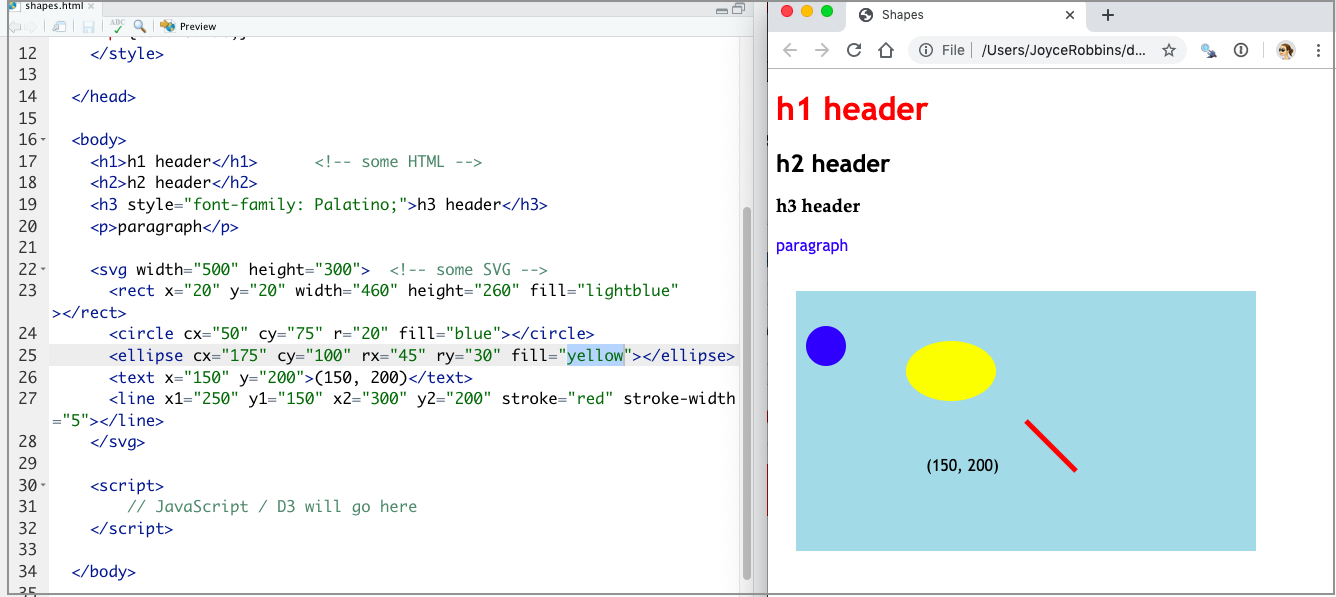
\includegraphics[width=0.8\linewidth]{images/editor_chrome} \end{center}

\begin{enumerate}
\def\labelenumi{\arabic{enumi}.}
\item
  Add an additional circle to the svg.
\item
  Add styling to the internal style sheet to style circles.
\item
  Add two additional paragraphs use the \texttt{\textless{}p\textgreater{}} tag.
\item
  Add an ID attribute to one of the circles.
\item
  Add a class attribute to two of the \texttt{\textless{}p\textgreater{}} tags.
\item
  Use the internal style sheet to style paragraphs of the class you created in 5.
\item
  Adjust additional elements as desired.
\end{enumerate}

\hypertarget{d3console}{%
\chapter{D3 in the Console }\label{d3console}}

\hypertarget{selections}{%
\section{Selections }\label{selections}}

\hypertarget{select-by-tag}{%
\subsection{Select by tag}\label{select-by-tag}}

The ability to select elements on a page is key to being able to manipulate them. \texttt{d3.select()} will select the first match; \texttt{d3.selectAll()} will select all matches.

\begin{Shaded}
\begin{Highlighting}[]
\VariableTok{d3}\NormalTok{.}\AttributeTok{select}\NormalTok{(}\StringTok{"svg"}\NormalTok{).}\AttributeTok{select}\NormalTok{(}\StringTok{"circle"}\NormalTok{)}\OperatorTok{;}
\end{Highlighting}
\end{Shaded}

selects the first circle in the order in which circles appear in the \texttt{\textless{}svg\textgreater{}} grouping. If there were more than one circle we could select them all with:

\begin{Shaded}
\begin{Highlighting}[]
\VariableTok{d3}\NormalTok{.}\AttributeTok{select}\NormalTok{(}\StringTok{"svg"}\NormalTok{).}\AttributeTok{selectAll}\NormalTok{(}\StringTok{"circle"}\NormalTok{)}\OperatorTok{;}
\end{Highlighting}
\end{Shaded}

We can select HTML elements by tag in the same way:

\begin{Shaded}
\begin{Highlighting}[]
\VariableTok{d3}\NormalTok{.}\AttributeTok{select}\NormalTok{(}\StringTok{"body"}\NormalTok{).}\AttributeTok{select}\NormalTok{(}\StringTok{"h1"}\NormalTok{)}\OperatorTok{;}
\VariableTok{d3}\NormalTok{.}\AttributeTok{select}\NormalTok{(}\StringTok{"body"}\NormalTok{).}\AttributeTok{selectAll}\NormalTok{(}\StringTok{"h1"}\NormalTok{)}\OperatorTok{;}
\end{Highlighting}
\end{Shaded}

\hypertarget{select-by-class}{%
\subsection{Select by class}\label{select-by-class}}

Classes are selected by adding a ``.'' before the class name:

\begin{Shaded}
\begin{Highlighting}[]
\VariableTok{d3}\NormalTok{.}\AttributeTok{select}\NormalTok{(}\StringTok{"svg"}\NormalTok{).}\AttributeTok{selectAll}\NormalTok{(}\StringTok{"circle.apple"}\NormalTok{)}
\end{Highlighting}
\end{Shaded}

This provides one method of selecting a certain collection of elements of the same type.

\hypertarget{select-by-id}{%
\subsection{Select by ID}\label{select-by-id}}

IDs differ from classes in that they are unique identifies. IDs are selected by adding a ``\#'' before the ID:

\begin{Shaded}
\begin{Highlighting}[]
\VariableTok{d3}\NormalTok{.}\AttributeTok{select}\NormalTok{(}\StringTok{"svg"}\NormalTok{).}\AttributeTok{select}\NormalTok{(}\StringTok{"circle#henry"}\NormalTok{)}\OperatorTok{;}
\end{Highlighting}
\end{Shaded}

\hypertarget{store-selections}{%
\subsection{Store selections}\label{store-selections}}

It is often helpful to store selections for later use. Here we store the svg selection in \texttt{mysvg}:

\begin{Shaded}
\begin{Highlighting}[]
\KeywordTok{var}\NormalTok{ mysvg }\OperatorTok{=} \VariableTok{d3}\NormalTok{.}\AttributeTok{select}\NormalTok{(}\StringTok{"svg"}\NormalTok{)}\OperatorTok{;}
\end{Highlighting}
\end{Shaded}

\begin{quote}
 \emph{The JavaScript community is moving toward using \texttt{let} and \texttt{const} instead of \texttt{var}; we, however, will stick with \texttt{var} to be consistent with }IDVW\emph{. Of course you're welcome to use \texttt{const} and \texttt{let} instead, and if so, may find these articles helpful: \href{https://madhatted.com/2016/1/25/let-it-be}{Let It Be - How to declare JavaScript variables} and \href{https://mathiasbynens.be/notes/es6-const}{ES2015 const is not about immutability}.}
\end{quote}

Store circle selection in a variable:

\begin{Shaded}
\begin{Highlighting}[]
\KeywordTok{var}\NormalTok{ svg }\OperatorTok{=} \VariableTok{d3}\NormalTok{.}\AttributeTok{select}\NormalTok{(}\StringTok{"svg"}\NormalTok{)}\OperatorTok{;}

\KeywordTok{var}\NormalTok{ circ }\OperatorTok{=} \VariableTok{svg}\NormalTok{.}\AttributeTok{selectAll}\NormalTok{(}\StringTok{"circle"}\NormalTok{)}\OperatorTok{;}
\end{Highlighting}
\end{Shaded}

\hypertarget{modify-existing-elements}{%
\section{Modify existing elements }\label{modify-existing-elements}}

Try out the code in this section with a downloaded copy of \href{https://raw.githubusercontent.com/jtr13/d3book/master/code/five_green_circles.html}{five\_green\_circles.html} opened in Chrome and the Console visible.

\hypertarget{modifying-attributes}{%
\subsection{Modifying attributes}\label{modifying-attributes}}

\href{https://github.com/d3/d3-selection/blob/v1.4.0/README.md\#selection_attr}{link to get or set attribute API}

\begin{Shaded}
\begin{Highlighting}[]
\VariableTok{d3}\NormalTok{.}\AttributeTok{select}\NormalTok{(}\StringTok{"circle"}\NormalTok{).}\AttributeTok{attr}\NormalTok{(}\StringTok{"r"}\NormalTok{)}\OperatorTok{;}           \CommentTok{// see radius}

\VariableTok{d3}\NormalTok{.}\AttributeTok{select}\NormalTok{(}\StringTok{"circle"}\NormalTok{).}\AttributeTok{attr}\NormalTok{(}\StringTok{"r"}\OperatorTok{,} \StringTok{"10"}\NormalTok{)}\OperatorTok{;}     \CommentTok{// set radius to 10}
\end{Highlighting}
\end{Shaded}

\hypertarget{modifying-styles}{%
\subsection{Modifying styles}\label{modifying-styles}}

\href{https://github.com/d3/d3-selection/blob/v1.4.0/README.md\#selection_style}{link to get or set style API}

\begin{Shaded}
\begin{Highlighting}[]
\VariableTok{d3}\NormalTok{.}\AttributeTok{select}\NormalTok{(}\StringTok{"h1"}\NormalTok{).}\AttributeTok{style}\NormalTok{(}\StringTok{"color"}\NormalTok{)}\OperatorTok{;}

\VariableTok{d3}\NormalTok{.}\AttributeTok{select}\NormalTok{(}\StringTok{"h1"}\NormalTok{).}\AttributeTok{style}\NormalTok{(}\StringTok{"color"}\OperatorTok{,} \StringTok{"blue"}\NormalTok{)}\OperatorTok{;}
\end{Highlighting}
\end{Shaded}

\begin{quote}
 \emph{It is often difficult to remember whether to use \texttt{.attr()} or \texttt{.style()} In general, properties such as position on the SVG, class, and ID are }attributes\emph{, while decorative properties such as color, font, font size, etc. are }styles\emph{. However, in some cases, you can use either. For example, the following both make the circle blue:}
\end{quote}

\begin{Shaded}
\begin{Highlighting}[]
\VariableTok{d3}\NormalTok{.}\AttributeTok{select}\NormalTok{(}\StringTok{"circle"}\NormalTok{).}\AttributeTok{attr}\NormalTok{(}\StringTok{"fill"}\OperatorTok{,} \StringTok{"blue"}\NormalTok{)}\OperatorTok{;}

\VariableTok{d3}\NormalTok{.}\AttributeTok{select}\NormalTok{(}\StringTok{"circle"}\NormalTok{).}\AttributeTok{style}\NormalTok{(}\StringTok{"fill"}\OperatorTok{,} \StringTok{"blue"}\NormalTok{)}\OperatorTok{;}
\end{Highlighting}
\end{Shaded}

\emph{The first will add a \texttt{fill="blue"} attribute to the \texttt{\textless{}circle\textgreater{}} tag, while the latter will add \texttt{style="fill:\ blue;"}. All is well and good until you find yourself with both in the same tag, in which case the \texttt{style} property will take precedence. The bottom line: don't mix the two options because it can cause problems.}

\begin{quote}
 \emph{To further complicate matters, \texttt{.style()} is just shorthand for \texttt{.attr("style",\ "...")} so the following are in fact equivalent:}
\end{quote}

\begin{Shaded}
\begin{Highlighting}[]
\VariableTok{d3}\NormalTok{.}\AttributeTok{select}\NormalTok{(}\StringTok{"circle"}\NormalTok{).}\AttributeTok{style}\NormalTok{(}\StringTok{"fill"}\OperatorTok{,} \StringTok{"blue"}\NormalTok{)}\OperatorTok{;}

\VariableTok{d3}\NormalTok{.}\AttributeTok{select}\NormalTok{(}\StringTok{"circle"}\NormalTok{).}\AttributeTok{attr}\NormalTok{(}\StringTok{"style"}\OperatorTok{,} \StringTok{"fill: blue;"}\NormalTok{)}\OperatorTok{;}
\end{Highlighting}
\end{Shaded}

\emph{In other words, style is an attribute!}

\hypertarget{modifying-text}{%
\subsection{Modifying text}\label{modifying-text}}

This section is interactive. Hover over code as directed to observe effects.

\hypertarget{html-text}{%
\subsubsection*{HTML text}\label{html-text}}
\addcontentsline{toc}{subsubsection}{HTML text}

\begin{Shaded}
\begin{Highlighting}[]
\KeywordTok{<p}\OtherTok{ id=}\StringTok{"typo"}\OtherTok{ class=}\StringTok{"fancy"}\KeywordTok{>}\NormalTok{Manhatten}\KeywordTok{</p>}
\end{Highlighting}
\end{Shaded}

Manhatten

Hover to execute this code (and fix the typo):

\hypertarget{fixtypo}{}
\begin{Shaded}
\begin{Highlighting}[]
\VariableTok{d3}\NormalTok{.}\AttributeTok{select}\NormalTok{(}\StringTok{"#typo"}\NormalTok{).}\AttributeTok{text}\NormalTok{(}\StringTok{"Manhattan"}\NormalTok{)}\OperatorTok{;}
\end{Highlighting}
\end{Shaded}

\hypertarget{svg-text}{%
\subsubsection*{SVG text}\label{svg-text}}
\addcontentsline{toc}{subsubsection}{SVG text}

\begin{Shaded}
\begin{Highlighting}[]
\KeywordTok{<svg}\OtherTok{ width=}\StringTok{"500"}\OtherTok{ height=}\StringTok{"100"}\KeywordTok{>}
  \KeywordTok{<rect}\OtherTok{ width=}\StringTok{"500"}\OtherTok{ height=}\StringTok{"100"}\OtherTok{ fill=}\StringTok{"#326EA4"}\KeywordTok{></rect>}
  \KeywordTok{<text}\OtherTok{ id=}\StringTok{"svgtypo"}\OtherTok{ x=}\StringTok{"50"}\OtherTok{ y=}\StringTok{"70"}\OtherTok{ fill=}\StringTok{"white"}\OtherTok{ font-weight=}\StringTok{"bold"}\OtherTok{ font-size=}\StringTok{"40px"}\KeywordTok{>}
\NormalTok{     Web scrapping is fun.}\KeywordTok{</text>}
\KeywordTok{</svg>}  
\end{Highlighting}
\end{Shaded}

Web scrapping is fun.

Hover to execute this code (and fix the typo):

\hypertarget{fixsvgtypo}{}
\begin{Shaded}
\begin{Highlighting}[]
\VariableTok{d3}\NormalTok{.}\AttributeTok{select}\NormalTok{(}\StringTok{"#svgtypo"}\NormalTok{).}\AttributeTok{text}\NormalTok{(}\StringTok{"Web scraping is fun."}\NormalTok{)}\OperatorTok{;}
\end{Highlighting}
\end{Shaded}

\begin{quote}
 \emph{The SVG \texttt{\textless{}text\textgreater{}} tag can be tricky. It differs from HTML text tags (\texttt{\textless{}p\textgreater{},\ \textless{}h1\textgreater{},\ \textless{}h2\textgreater{},} etc.) in that it has \texttt{x} and \texttt{y} attributes that allow you to position text on an SVG canvas. Unlike HTML, the fill attribute controls the color of the text. Compare:}
\end{quote}

\begin{Shaded}
\begin{Highlighting}[]
\VariableTok{d3}\NormalTok{.}\AttributeTok{select}\NormalTok{(}\StringTok{"p"}\NormalTok{).}\AttributeTok{style}\NormalTok{(}\StringTok{"color"}\OperatorTok{,} \StringTok{"red"}\NormalTok{)}\OperatorTok{;}   \CommentTok{// HTML}

\VariableTok{d3}\NormalTok{.}\AttributeTok{select}\NormalTok{(}\StringTok{"text"}\NormalTok{).}\AttributeTok{attr}\NormalTok{(}\StringTok{"fill"}\OperatorTok{,} \StringTok{"red"}\NormalTok{)}\OperatorTok{;}  \CommentTok{// SVG}
\end{Highlighting}
\end{Shaded}

\hypertarget{moving-svg-text}{%
\subsection{Moving SVG text}\label{moving-svg-text}}

\begin{Shaded}
\begin{Highlighting}[]
\KeywordTok{<svg}\OtherTok{ width=}\StringTok{"600"}\OtherTok{ height=}\StringTok{"100"}\KeywordTok{>}
  \KeywordTok{<rect}\OtherTok{ width=}\StringTok{"600"}\OtherTok{ height=}\StringTok{"100"}\OtherTok{ fill=}\StringTok{"#326EA4"}\KeywordTok{></rect>}
  \KeywordTok{<text}\OtherTok{ id=}\StringTok{"moveleft"}\OtherTok{ x=}\StringTok{"200"}\OtherTok{ y=}\StringTok{"70"}\OtherTok{ fill=}\StringTok{"white"}\OtherTok{ font-weight=}\StringTok{"bold"}\OtherTok{ font-size=}\StringTok{"40px"}\KeywordTok{>}
\NormalTok{      I want to move left.}\KeywordTok{</text>}
\KeywordTok{</svg>}  
\end{Highlighting}
\end{Shaded}

I want to move left.

Hover to execute this code:

\hypertarget{move}{}
\begin{Shaded}
\begin{Highlighting}[]
\VariableTok{d3}\NormalTok{.}\AttributeTok{select}\NormalTok{(}\StringTok{"#moveleft"}\NormalTok{).}\AttributeTok{attr}\NormalTok{(}\StringTok{"x"}\OperatorTok{,} \StringTok{"20"}\NormalTok{).}\AttributeTok{text}\NormalTok{(}\StringTok{"Thanks, now I'm happy!"}\NormalTok{)}\OperatorTok{;}
\end{Highlighting}
\end{Shaded}

\hypertarget{adding-elements}{%
\section{Adding elements }\label{adding-elements}}

\hypertarget{html-1}{%
\subsection{HTML}\label{html-1}}

Continue trying out code with \texttt{five\_green\_circles.html} open in Chrome.

The following adds a \texttt{\textless{}p\textgreater{}} tag but doesn't change how the page looks, since there's no text associated with it.

\begin{Shaded}
\begin{Highlighting}[]
\VariableTok{d3}\NormalTok{.}\AttributeTok{select}\NormalTok{(}\StringTok{"body"}\NormalTok{).}\AttributeTok{append}\NormalTok{(}\StringTok{"p"}\NormalTok{)}\OperatorTok{;}
\end{Highlighting}
\end{Shaded}

To add text, use \texttt{.text()}:

\begin{Shaded}
\begin{Highlighting}[]
\VariableTok{d3}\NormalTok{.}\AttributeTok{select}\NormalTok{(}\StringTok{"body"}\NormalTok{).}\AttributeTok{append}\NormalTok{(}\StringTok{"p"}\NormalTok{).}\AttributeTok{text}\NormalTok{(}\StringTok{"This is a complete sentence."}\NormalTok{)}\OperatorTok{;}
\end{Highlighting}
\end{Shaded}

\begin{quote}
 \emph{To debug adding an element, go to the Elements tab to see what was added and where. If an element is in the wrong place in the HTML tree, it will not be visible.}
\end{quote}

\hypertarget{svg-1}{%
\subsection{SVG}\label{svg-1}}

Likewise, here we add a \texttt{\textless{}circle\textgreater{}} to the \texttt{\textless{}svg\textgreater{}}, but we can't see it since it has no attributes.

\begin{Shaded}
\begin{Highlighting}[]
\VariableTok{d3}\NormalTok{.}\AttributeTok{select}\NormalTok{(}\StringTok{"svg"}\NormalTok{).}\AttributeTok{append}\NormalTok{(}\StringTok{"circle"}\NormalTok{)}\OperatorTok{;}
\end{Highlighting}
\end{Shaded}

Adding attributes will create visible circles:

\begin{Shaded}
\begin{Highlighting}[]
\VariableTok{d3}\NormalTok{.}\AttributeTok{select}\NormalTok{(}\StringTok{"svg"}\NormalTok{).}\AttributeTok{append}\NormalTok{(}\StringTok{"rect"}\NormalTok{).}\AttributeTok{attr}\NormalTok{(}\StringTok{"x"}\OperatorTok{,} \StringTok{"0"}\NormalTok{).}\AttributeTok{attr}\NormalTok{(}\StringTok{"y"}\OperatorTok{,} \StringTok{"0"}\NormalTok{)}
\NormalTok{    .}\AttributeTok{attr}\NormalTok{(}\StringTok{"width"}\OperatorTok{,} \StringTok{"500"}\NormalTok{).}\AttributeTok{attr}\NormalTok{(}\StringTok{"height"}\OperatorTok{,} \StringTok{"400"}\NormalTok{).}\AttributeTok{attr}\NormalTok{(}\StringTok{"fill"}\OperatorTok{,} \StringTok{"lightblue"}\NormalTok{)}\OperatorTok{;}
    
\VariableTok{d3}\NormalTok{.}\AttributeTok{select}\NormalTok{(}\StringTok{"svg"}\NormalTok{).}\AttributeTok{append}\NormalTok{(}\StringTok{"circle"}\NormalTok{).}\AttributeTok{attr}\NormalTok{(}\StringTok{"cx"}\OperatorTok{,} \StringTok{"200"}\NormalTok{)}
\NormalTok{    .}\AttributeTok{attr}\NormalTok{(}\StringTok{"cy"}\OperatorTok{,} \StringTok{"100"}\NormalTok{).}\AttributeTok{attr}\NormalTok{(}\StringTok{"r"}\OperatorTok{,} \StringTok{"25"}\NormalTok{).}\AttributeTok{attr}\NormalTok{(}\StringTok{"fill"}\OperatorTok{,} \StringTok{"orange"}\NormalTok{)}\OperatorTok{;}
    
\VariableTok{d3}\NormalTok{.}\AttributeTok{select}\NormalTok{(}\StringTok{"svg"}\NormalTok{).}\AttributeTok{append}\NormalTok{(}\StringTok{"circle"}\NormalTok{).}\AttributeTok{attr}\NormalTok{(}\StringTok{"cx"}\OperatorTok{,} \StringTok{"300"}\NormalTok{)}
\NormalTok{    .}\AttributeTok{attr}\NormalTok{(}\StringTok{"cy"}\OperatorTok{,} \StringTok{"150"}\NormalTok{).}\AttributeTok{attr}\NormalTok{(}\StringTok{"r"}\OperatorTok{,} \StringTok{"25"}\NormalTok{).}\AttributeTok{attr}\NormalTok{(}\StringTok{"fill"}\OperatorTok{,} \StringTok{"red"}\NormalTok{)}\OperatorTok{;}  
\end{Highlighting}
\end{Shaded}

We can use a saved selection to assist in creating a new element:

\begin{Shaded}
\begin{Highlighting}[]
\NormalTok{mysvg }\OperatorTok{=} \VariableTok{d3}\NormalTok{.}\AttributeTok{select}\NormalTok{(}\StringTok{"svg"}\NormalTok{)}\OperatorTok{;}

\VariableTok{mysvg}\NormalTok{.}\AttributeTok{append}\NormalTok{(}\StringTok{"circle"}\NormalTok{).}\AttributeTok{attr}\NormalTok{(}\StringTok{"cx"}\OperatorTok{,} \StringTok{"250"}\NormalTok{).}\AttributeTok{attr}\NormalTok{(}\StringTok{"cy"}\OperatorTok{,} \StringTok{"250"}\NormalTok{).}\AttributeTok{attr}\NormalTok{(}\StringTok{"r"}\OperatorTok{,} \StringTok{"50"}\NormalTok{)}
\NormalTok{  .}\AttributeTok{attr}\NormalTok{(}\StringTok{"fill"}\OperatorTok{,} \StringTok{"red"}\NormalTok{)}\OperatorTok{;}
\end{Highlighting}
\end{Shaded}

\hypertarget{removing-elements}{%
\section{Removing elements }\label{removing-elements}}

These methods will remove matching elements in order, starting with the first find in the document.

\hypertarget{html-2}{%
\subsection{HTML}\label{html-2}}

\begin{Shaded}
\begin{Highlighting}[]
\VariableTok{d3}\NormalTok{.}\AttributeTok{select}\NormalTok{(}\StringTok{"p"}\NormalTok{).}\AttributeTok{remove}\NormalTok{()}\OperatorTok{;}
\end{Highlighting}
\end{Shaded}

\hypertarget{svg-2}{%
\subsection{SVG}\label{svg-2}}

\begin{Shaded}
\begin{Highlighting}[]
\VariableTok{d3}\NormalTok{.}\AttributeTok{select}\NormalTok{(}\StringTok{"svg"}\NormalTok{).}\AttributeTok{select}\NormalTok{(}\StringTok{"circle"}\NormalTok{).}\AttributeTok{remove}\NormalTok{()}\OperatorTok{;}

\VariableTok{d3}\NormalTok{.}\AttributeTok{select}\NormalTok{(}\StringTok{"svg"}\NormalTok{).}\AttributeTok{selectAll}\NormalTok{(}\StringTok{"circle"}\NormalTok{).}\AttributeTok{remove}\NormalTok{()}\OperatorTok{;}
\end{Highlighting}
\end{Shaded}

\hypertarget{exercise-1}{%
\section{Exercise }\label{exercise-1}}

Download and open a fresh copy of \href{https://raw.githubusercontent.com/jtr13/d3book/master/code/five_green_circles.html}{five\_green\_circles.html} in Chrome with Developer Tools open. Do the following in the Console with D3:

\begin{enumerate}
\def\labelenumi{\arabic{enumi}.}
\item
  Select the circle with ID ``henry'' and make it blue.
\item
  Select all circles of ``apple'' class make them red.
\item
  Select the first circle and add an orange border (``stroke''), and stroke width (``stroke-width'') of 5.
\item
  Select all circles of ``apple'' class and move them to the middle of the svg.
\end{enumerate}

\hypertarget{binding-data-finally}{%
\section{\texorpdfstring{Binding data\ldots{} \emph{finally!} }{Binding data\ldots{} finally! }}\label{binding-data-finally}}

To follow along with the code in this section, download and open a fresh copy of \href{https://raw.githubusercontent.com/jtr13/d3book/master/code/six_blue_circles.html}{six\_blue\_circles.html}.

Bind data:

\begin{Shaded}
\begin{Highlighting}[]
\VariableTok{d3}\NormalTok{.}\AttributeTok{select}\NormalTok{(}\StringTok{"svg"}\NormalTok{).}\AttributeTok{selectAll}\NormalTok{(}\StringTok{"circle"}\NormalTok{).}\AttributeTok{data}\NormalTok{([}\DecValTok{90}\OperatorTok{,} \DecValTok{230}\OperatorTok{,} \DecValTok{140}\OperatorTok{,} \DecValTok{75}\OperatorTok{,} \DecValTok{180}\OperatorTok{,} \DecValTok{25}\NormalTok{])}\OperatorTok{;}
\end{Highlighting}
\end{Shaded}

Check data binding:

\begin{Shaded}
\begin{Highlighting}[]
\VariableTok{d3}\NormalTok{.}\AttributeTok{select}\NormalTok{(}\StringTok{"svg"}\NormalTok{).}\AttributeTok{selectAll}\NormalTok{(}\StringTok{"circle"}\NormalTok{).}\AttributeTok{data}\NormalTok{()}\OperatorTok{;}
\end{Highlighting}
\end{Shaded}

Set x-coordinate of each circle to data value using arrow function:

\begin{Shaded}
\begin{Highlighting}[]
\VariableTok{d3}\NormalTok{.}\AttributeTok{select}\NormalTok{(}\StringTok{"svg"}\NormalTok{).}\AttributeTok{selectAll}\NormalTok{(}\StringTok{"circle"}\NormalTok{).}\AttributeTok{attr}\NormalTok{(}\StringTok{"cx"}\OperatorTok{,}\NormalTok{ d }\OperatorTok{=>}\NormalTok{ d)}\OperatorTok{;}
\end{Highlighting}
\end{Shaded}

Set x-coordinate of each circle to data value with a JavaScript function:

\begin{Shaded}
\begin{Highlighting}[]
\VariableTok{d3}\NormalTok{.}\AttributeTok{select}\NormalTok{(}\StringTok{"svg"}\NormalTok{).}\AttributeTok{selectAll}\NormalTok{(}\StringTok{"circle"}\NormalTok{).}\AttributeTok{attr}\NormalTok{(}\StringTok{"cx"}\OperatorTok{,} \KeywordTok{function}\NormalTok{(d) }\OperatorTok{\{}\ControlFlowTok{return}\NormalTok{ d}\OperatorTok{;\}}\NormalTok{)}\OperatorTok{;}
\end{Highlighting}
\end{Shaded}

We'll bind a new set of data to the circles, this time storying the dataset in a variable:

\begin{Shaded}
\begin{Highlighting}[]
\KeywordTok{var}\NormalTok{ dataset }\OperatorTok{=}\NormalTok{ [}\DecValTok{50}\OperatorTok{,} \DecValTok{80}\OperatorTok{,} \DecValTok{110}\OperatorTok{,} \DecValTok{140}\OperatorTok{,} \DecValTok{170}\OperatorTok{,} \DecValTok{200}\NormalTok{]}\OperatorTok{;}
\end{Highlighting}
\end{Shaded}

We'll also store a selection of all circles before binding the data:

\begin{Shaded}
\begin{Highlighting}[]
\NormalTok{circ }\OperatorTok{=} \VariableTok{d3}\NormalTok{.}\AttributeTok{select}\NormalTok{(}\StringTok{"svg"}\NormalTok{).}\AttributeTok{selectAll}\NormalTok{(}\StringTok{"circle"}\NormalTok{)}\OperatorTok{;}
\end{Highlighting}
\end{Shaded}

And now, the data bind:

\begin{Shaded}
\begin{Highlighting}[]
\VariableTok{circ}\NormalTok{.}\AttributeTok{data}\NormalTok{(dataset)}\OperatorTok{;}
\end{Highlighting}
\end{Shaded}

Nothing appears to have happened; the circles remain the same and there is no evidence of any changes looking at the circles in the DOM (see Elements tab).

We can check that the data are indeed bound with:

\begin{Shaded}
\begin{Highlighting}[]
\VariableTok{circ}\NormalTok{.}\AttributeTok{data}\NormalTok{()}\OperatorTok{;}  \CommentTok{// now we see data}
\end{Highlighting}
\end{Shaded}

Modify elements w/ stored selections, bound data:

\begin{Shaded}
\begin{Highlighting}[]
\VariableTok{circ}\NormalTok{.}\AttributeTok{attr}\NormalTok{(}\StringTok{"cx"}\OperatorTok{,} \KeywordTok{function}\NormalTok{(d) }\OperatorTok{\{}\ControlFlowTok{return}\NormalTok{ d}\OperatorTok{;\}}\NormalTok{)}\OperatorTok{;}

\VariableTok{circ}\NormalTok{.}\AttributeTok{attr}\NormalTok{(}\StringTok{"cx"}\OperatorTok{,} \KeywordTok{function}\NormalTok{(d) }\OperatorTok{\{}\ControlFlowTok{return}\NormalTok{ d/}\DecValTok{2}\OperatorTok{;\}}\NormalTok{)}\OperatorTok{;}

\VariableTok{circ}\NormalTok{.}\AttributeTok{attr}\NormalTok{(}\StringTok{"cx"}\OperatorTok{,} \KeywordTok{function}\NormalTok{(d) }\OperatorTok{\{}\ControlFlowTok{return}\NormalTok{ d/}\DecValTok{4}\OperatorTok{;\}}\NormalTok{).}\AttributeTok{attr}\NormalTok{(}\StringTok{"r"}\OperatorTok{,} \StringTok{"10"}\NormalTok{)}\OperatorTok{;}
\end{Highlighting}
\end{Shaded}

Same as above, using arrow functions:

\begin{Shaded}
\begin{Highlighting}[]
\VariableTok{circ}\NormalTok{.}\AttributeTok{attr}\NormalTok{(}\StringTok{"cx"}\OperatorTok{,}\NormalTok{ d }\OperatorTok{=>}\NormalTok{ d)}\OperatorTok{;}

\VariableTok{circ}\NormalTok{.}\AttributeTok{attr}\NormalTok{(}\StringTok{"cx"}\OperatorTok{,}\NormalTok{ d }\OperatorTok{=>}\NormalTok{ d/}\DecValTok{2}\NormalTok{)}\OperatorTok{;}

\VariableTok{circ}\NormalTok{.}\AttributeTok{attr}\NormalTok{(}\StringTok{"r"}\OperatorTok{,}\NormalTok{ d }\OperatorTok{=>}\NormalTok{ d/}\DecValTok{4}\NormalTok{).}\AttributeTok{attr}\NormalTok{(}\StringTok{"r"}\OperatorTok{,} \StringTok{"10"}\NormalTok{)}\OperatorTok{;}
\end{Highlighting}
\end{Shaded}

Note that if we bind a new set of data to the DOM elements, the original set will be overwritten:

\begin{Shaded}
\begin{Highlighting}[]
\KeywordTok{var}\NormalTok{ newdata }\OperatorTok{=}\NormalTok{ [}\DecValTok{145}\OperatorTok{,} \DecValTok{29}\OperatorTok{,} \DecValTok{53}\OperatorTok{,} \DecValTok{196}\OperatorTok{,} \DecValTok{200}\OperatorTok{,} \DecValTok{12}\NormalTok{]}\OperatorTok{;}

\VariableTok{circ}\NormalTok{.}\AttributeTok{data}\NormalTok{(newdata)}\OperatorTok{;}

\VariableTok{circ}\NormalTok{.}\AttributeTok{transition}\NormalTok{()}
\NormalTok{    .}\AttributeTok{duration}\NormalTok{(}\DecValTok{2000}\NormalTok{)}
\NormalTok{    .}\AttributeTok{attr}\NormalTok{(}\StringTok{"cx"}\OperatorTok{,}\NormalTok{ d }\OperatorTok{=>} \DecValTok{2}\OperatorTok{*}\NormalTok{d)}\OperatorTok{;}
\end{Highlighting}
\end{Shaded}

\hypertarget{exercise-2}{%
\section{Exercise }\label{exercise-2}}

With \texttt{six\_blue\_circles.html} open in Chrome, practice binding data to the circles and modifying the circles based on the data as in the examples above.

\hypertarget{more-chapters-coming-soon}{%
\chapter{More chapters coming soon }\label{more-chapters-coming-soon}}

via GIPHY

\bibliography{book.bib,packages.bib}


\end{document}
